\documentclass[11pt]{article}
\usepackage[margin=2.2cm]{geometry}
\usepackage{graphicx,booktabs,float,hyperref,amsmath}
\setlength{\parindent}{0pt}\setlength{\parskip}{6pt}
\newcommand{\img}[2]{\IfFileExists{#1}{\includegraphics[width=#2]{#1}}{\fbox{\parbox{0.9\textwidth}{\centering\vspace{2cm}Missing file: \texttt{\detokenize{#1}}\vspace{2cm}}}}}
\begin{document}
{\Large\bfseries CoE toy universe: geometry, Migkas fits and the observable list}\\[2pt]
Letter for Chris, 27 October 2026. Plain numbers from files on the working machine; no pass/fail calls.

\section{The geometry}
The model has one preferred direction: the line from us to the centre of expansion (CoE), at distance $D$. Our observable universe is a sphere of radius $R$ around us (Fig.~\ref{fig:geo}).
\begin{figure}[H]\centering\img{geometry_schematic.png}{0.85\textwidth}
\caption{Schematic: CoE, our position at distance $D$, our observable universe around us. Script \texttt{geometry\_schematic.py}.}\label{fig:geo}\end{figure}
Everything else is free to roll about the line to the CoE. The orange arc in Fig.~\ref{fig:arc} is the set of points as far from the CoE as we are, so they sit at the same CoE potential. Where it crosses the sky it gives the critical points P1, P2 and their antipodes.
\begin{figure}[H]\centering\img{chris_equal_distance_arc.png}{\textwidth}
\caption{Equal-distance arc and critical points P1, P2 (figure by C.~Alameddin).}\label{fig:arc}\end{figure}

\section{Migkas $A/A_{\rm all}$ and $B/B_{\rm all}$ vs angle}
Migkas et al.\ (2020, A\&A 636, A15) give the $L_X$--$T$ normalisation $A$ and slope $B$ in sliding $90^\circ$ cones; digitised at 71 points. Adjacent cones share most clusters, so $\chi^2$ is descriptive.

\textbf{$A$ and $B$ together} (Fig.~\ref{fig:AB}; source \texttt{migkas\_bars\_rotation\_summary.json}): sheet shell model with a one-cycle phase rotation, Amp $=\mp0.06$, $\varphi=0.35$\,rad. $R^2$ vs digitised points: A $0.446\to0.712$, B $0.483\to0.785$. Best shared $\varphi=0.522$\,rad: A 0.730, B 0.776. Against the sheet series: A $0.501\to0.739$, B $0.372\to0.733$.
\begin{figure}[H]\centering\img{R04_migkas_rotation.png}{0.8\textwidth}
\caption{$A/A_{\rm all}$ (top) and $B/B_{\rm all}$ (bottom) vs longitude with the rotated shell model. Script \texttt{R04\_migkas\_rotation.py}.}\label{fig:AB}\end{figure}

\textbf{$A/A_{\rm all}$, locked fit, residuals and their Fourier modes} (Fig.~\ref{fig:A}; computed by \texttt{A\_fit\_residual\_fourier.py}, values in \texttt{A\_fit\_residual\_fourier.json}). Locked CoE $\eta$-edge fit: $\chi^2=9.278$ (71 cones, mean of asymmetric errors), $r^2=0.745$ ($1-\mathrm{SS_{res}}/\mathrm{SS_{tot}}$; the paper quotes 0.748 with its own definition). Least-squares harmonics of the residuals, $m=1$--8, mean offset $-0.0032$. Largest modes: $m=1$ amplitude 0.0316 (50.2\% of residual harmonic power, peak at $l=125^\circ$); $m=3$ 0.0219 (24.2\%, first peak $l=59^\circ$); $m=5$ 0.0151 (11.4\%); $m=2$ 0.0130 (8.5\%). Modes 4, 6, 7, 8 together 5.8\%. For reference (\texttt{N2\_migkas\_cov.json}): profile refit at $D=34.96$\,Gpc $\chi^2=9.250$; isotropy 45.14; with overlap covariance CoE 3.88, isotropy 8.99, free dipole 6.90, dipole+quadrupole 5.20.
\begin{figure}[H]\centering\img{A_fit_residual_fourier.png}{0.88\textwidth}
\caption{Top: $A/A_{\rm all}$ and locked CoE fit. Middle: data minus fit, with the $m=1$--8 harmonic sum. Bottom: harmonic amplitudes with fractional power and first-peak longitude. Script \texttt{A\_fit\_residual\_fourier.py}.}\label{fig:A}\end{figure}

\section{Placing the model on the sky}
Placing the model needs the CoE direction (near $l\approx180^\circ$) and one roll about the CoE axis; expected roll band $45$--$80^\circ$, $60^\circ$ central. Fig.~\ref{fig:fig8} shows the orientation sequence and the Migkas 2D map overlays after rotation.
\clearpage\begin{figure}[H]\centering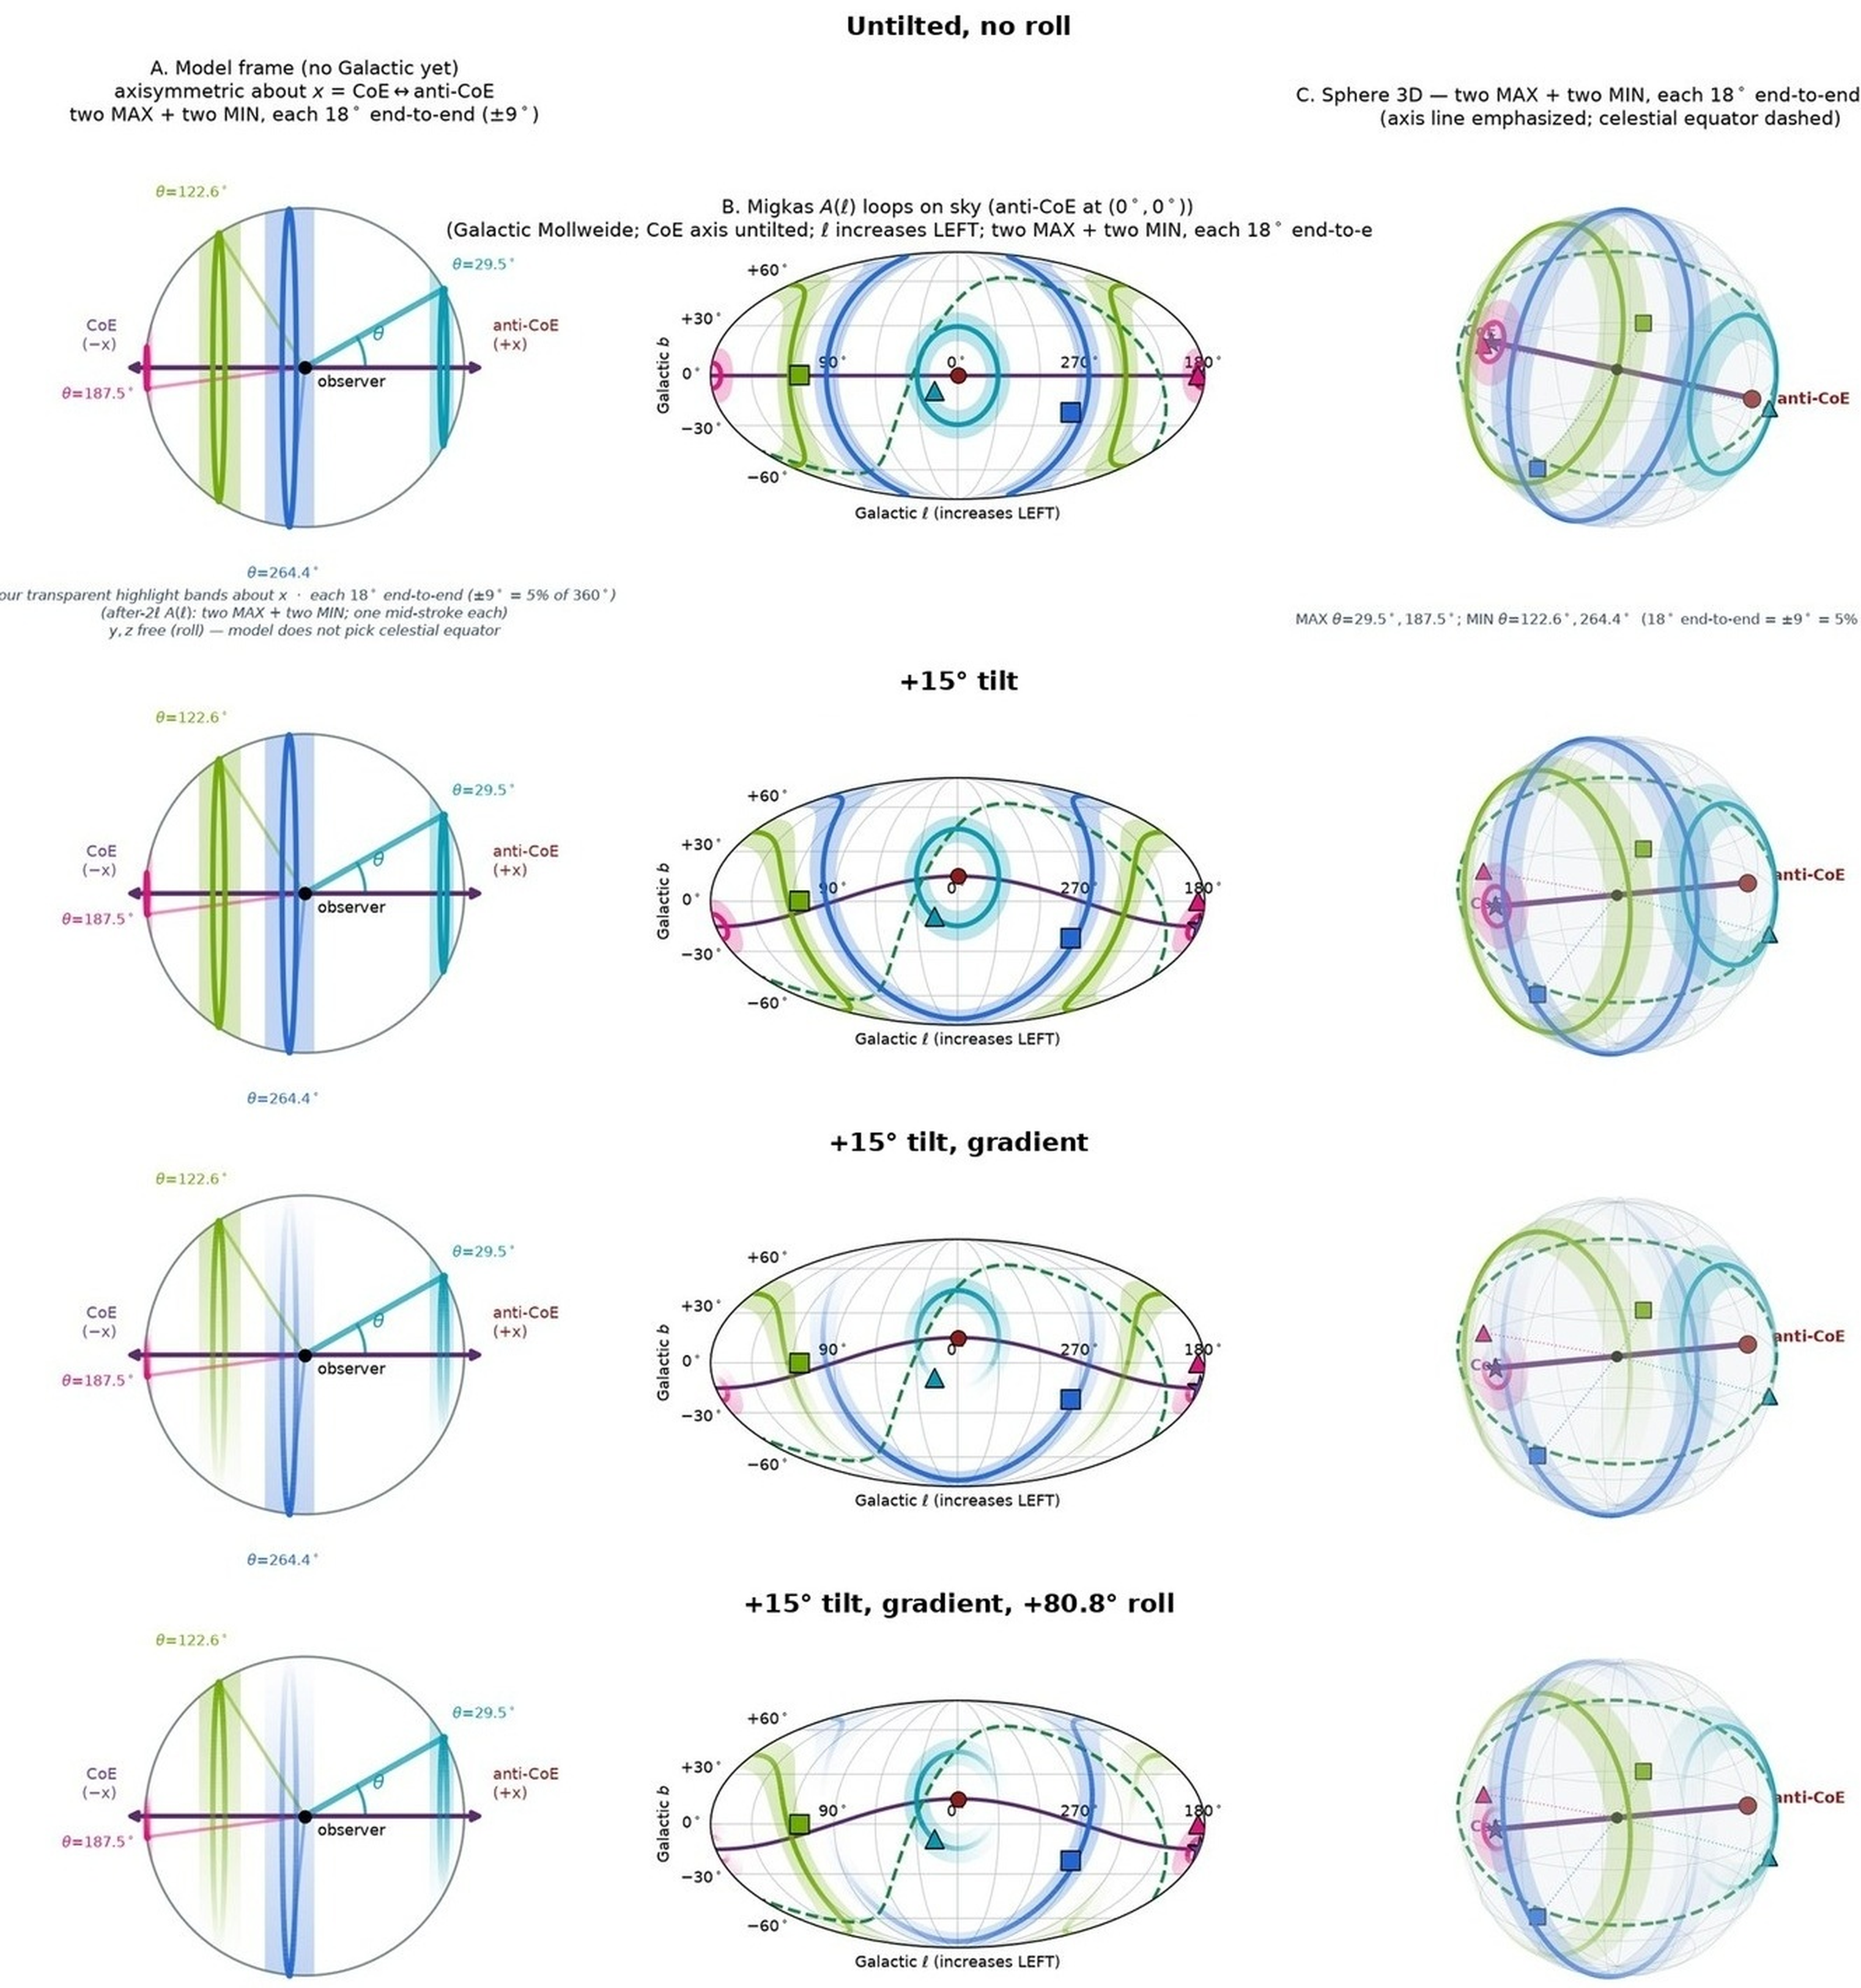
\includegraphics[width=\textwidth,height=0.88\textheight,keepaspectratio]{fig8_orientation_seq.png}\caption{Sky-orientation sequence (untilted, $+15^\circ$ tilt, radial gradient, $+80.8^\circ$ roll about the CoE axis). Maker \texttt{make\_fig05\_sky\_orientation.py}; split by \texttt{split\_fig8.py}.}\label{fig:fig8}\end{figure}
\clearpage\begin{figure}[H]\centering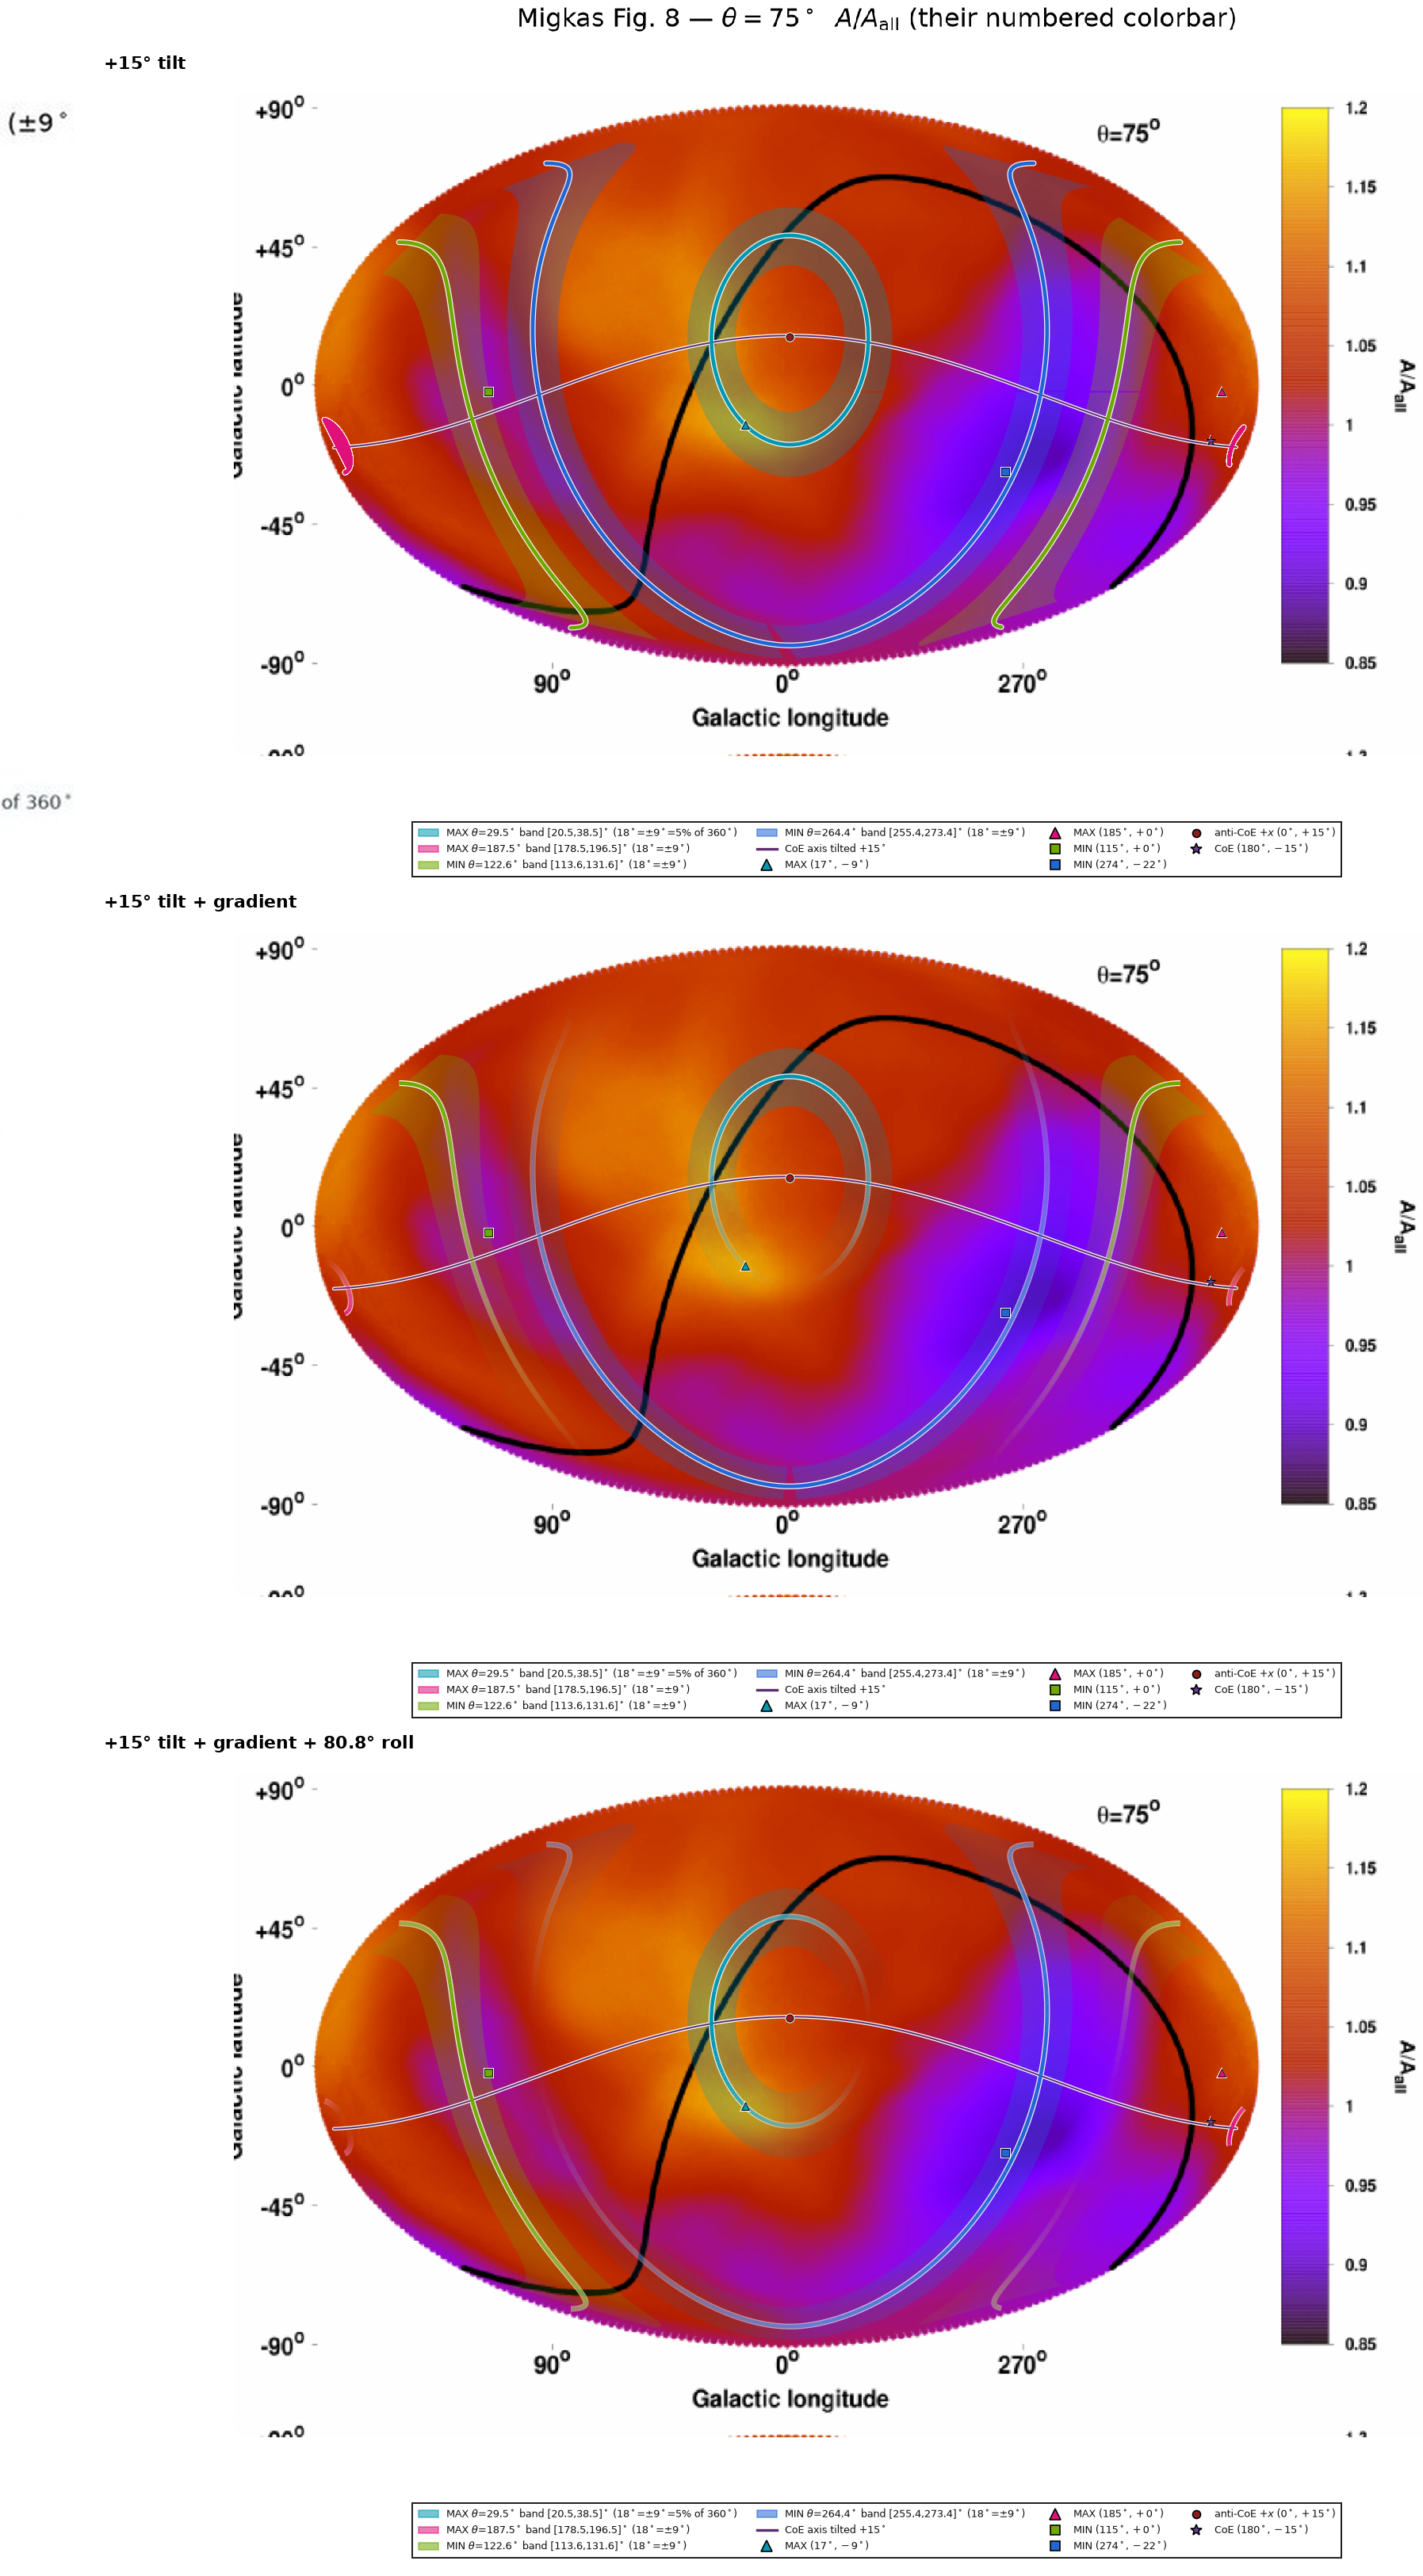
\includegraphics[width=\textwidth,height=0.88\textheight,keepaspectratio]{fig8_migkas_maps.png}\caption{Predicted MAX/MIN bands (two of each, $18^\circ$ wide) on the Migkas Fig.~8 2D map. Maker \texttt{make\_migkas\_fig8\_overlay\_matched.py}; split by \texttt{split\_fig8.py}.}\label{fig:fig8m}\end{figure}
\clearpage
The A and B residuals (after removing shared $n=1$--3 harmonics, $25^\circ$ running mean) are put on the sky with the CoE at $b=-15^\circ$ and roll $45^\circ$ (Fig.~\ref{fig:spots}).
\begin{figure}[H]\centering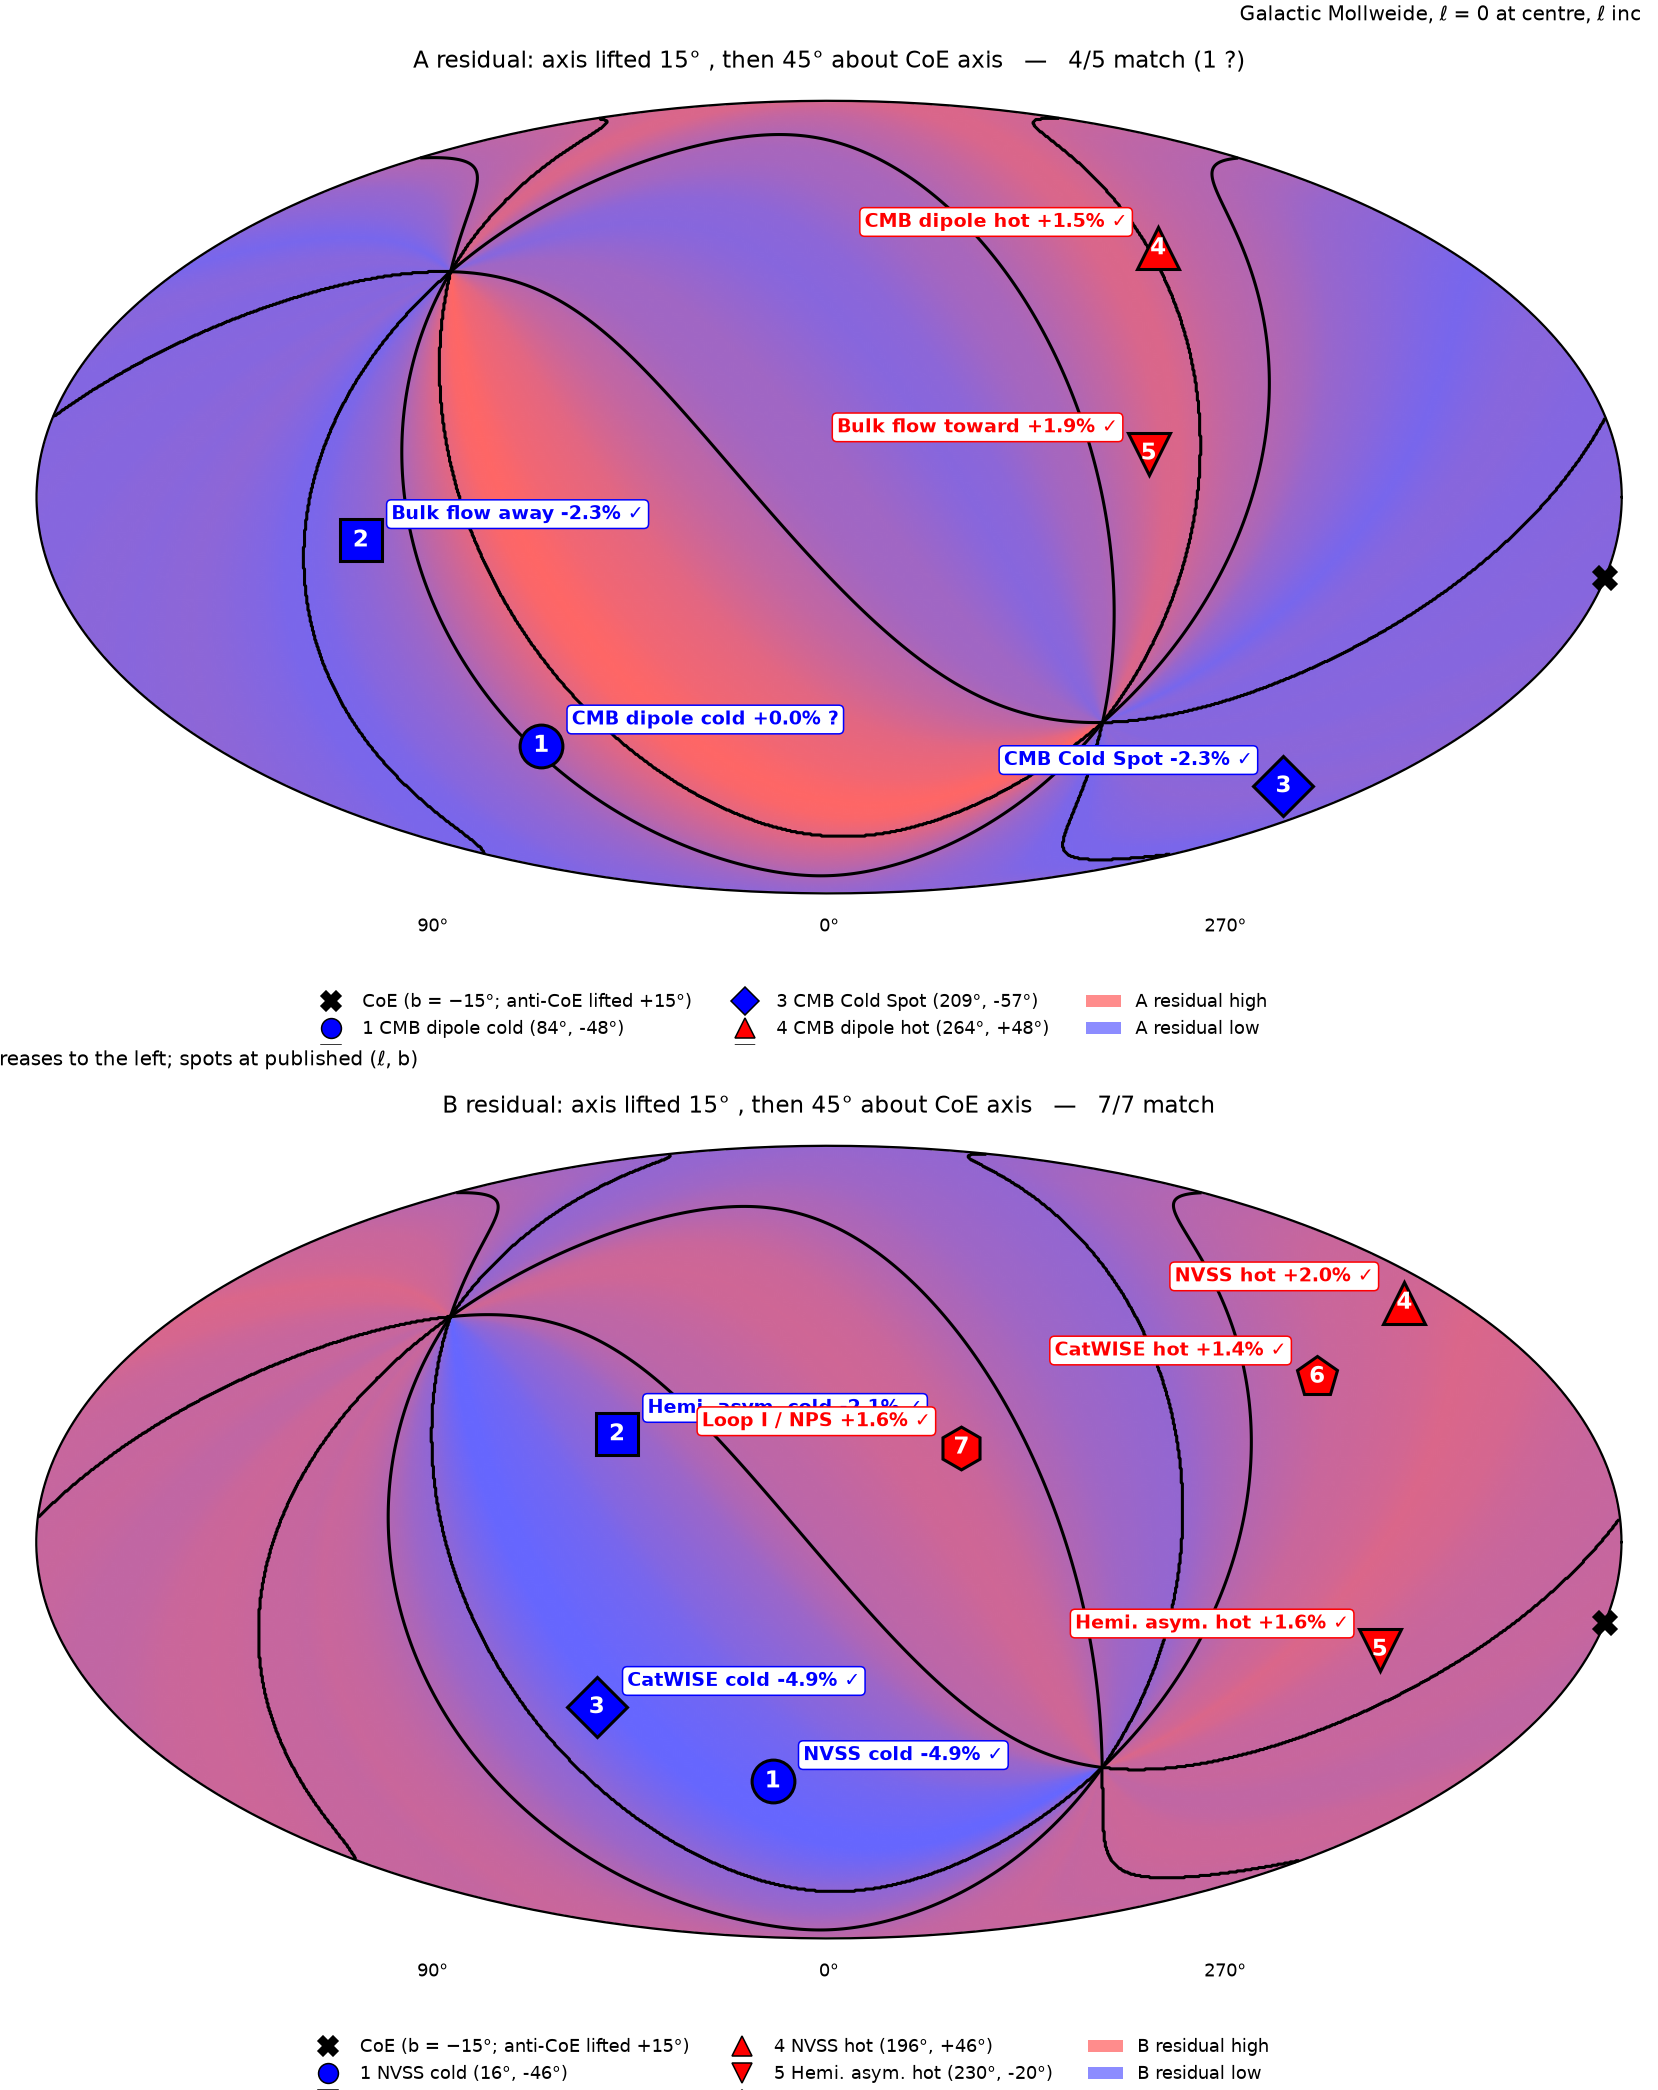
\includegraphics[width=\textwidth,height=0.85\textheight,keepaspectratio]{chris_AB_stacked.png}
\caption{A (top, spots 1--5) and B (bottom, spots 6--12) residual maps, CoE $b=-15^\circ$, roll $45^\circ$. Script \texttt{chris\_AB\_residual\_spots.py} (from \texttt{23\_sky\_mapA\_al.py}).}\label{fig:spots}\end{figure}\clearpage

\section{Where the dipoles land}
\begin{figure}[H]\centering\img{dipoles_sky_map.png}{0.9\textwidth}
\caption{Published dipole and anomaly directions (filled) and antipodes (open), with the model CoE direction $(180^\circ,-15^\circ)$. Migkas maximum anisotropy $(280^\circ,-15^\circ)$ from Migkas et al.\ (2021). Script \texttt{dipoles\_sky\_map.py}.}\label{fig:dip}\end{figure}

\section{The observables from the CoE point of view}
Each spot is tied to A (normalisation: distance, expansion, velocity) or B (slope: sample composition, foreground) from the physics before reading any sign. A hot spot needs residual $>0$, a cold spot $<0$. Bootstrap $1\sigma$ per spot is 3--6 points.

\begin{table}[H]\centering\small
\begin{tabular}{lllrl}\toprule
Observable & $(l,b)$ & tie & residual [\%] & sign\\\midrule
CMB dipole cold & $(84,-48)$ & A & $+0.024$ & on zero line\\
CMB dipole hot & $(264,+48)$ & A & $+1.538$ & matches\\
Bulk flow away & $(107,-8)$ & A & $-2.272$ & matches\\
Bulk flow toward & $(287,+8)$ & A & $+1.903$ & matches\\
CMB Cold Spot & $(209,-57)$ & A & $-2.331$ & matches\\
NVSS cold & $(16,-46)$ & B & $-4.872$ & matches\\
NVSS hot & $(196,+46)$ & B & $+2.028$ & matches\\
Hemispherical asym.\ cold & $(50,+20)$ & B & $-2.110$ & matches\\
Hemispherical asym.\ hot & $(230,-20)$ & B & $+1.621$ & matches\\
CatWISE cold & $(58,-31)$ & B & $-4.873$ & matches\\
CatWISE hot & $(238,+31)$ & B & $+1.388$ & matches\\
Loop I / NPS & $(329,+17.5)$ & B & $+1.598$ & matches\\\midrule
\multicolumn{5}{l}{Score: A 4/5, B 7/7, total 11/12 (source \texttt{lee\_results.json}, \texttt{R26\_29\_sky\_chain.py})}\\\bottomrule
\end{tabular}\end{table}

\textbf{CMB dipole} (A; our motion $\to$ distance/velocity). Planck 2018 I (A\&A 641, A1): $3.362$\,mK toward $(264.0^\circ,+48.3^\circ)$, i.e.\ $369.8$\,km/s. Hot pole $+1.54$, cold pole $+0.02$ (on the zero line, marked ``?'').

\textbf{Bulk flow} (A; recession velocity $\to$ distance). Watkins, Feldman \& Hudson 2009 (MNRAS 392, 743): $407\pm81$\,km/s toward $(287\pm9^\circ, 8\pm6^\circ)$. Toward $+1.90$, away $-2.27$.

\textbf{CMB Cold Spot} (A; Eridanus supervoid changes expansion along that sightline). Vielva et al.\ 2004 (ApJ 609, 22); Cruz et al.\ 2005 (MNRAS 356, 29): $\sim -70\,\mu$K at $(209^\circ,-57^\circ)$. Supervoid: Szapudi et al.\ 2015 (MNRAS 450, 288). Residual $-2.33$.

\textbf{NVSS radio dipole} (B; source density $\to$ sample). Singal 2011 (ApJL 742, L23); Rubart \& Schwarz 2013 (A\&A 555, A117): amplitude several times the kinematic expectation, direction near the CMB dipole. Cold $-4.87$, hot $+2.03$.

\textbf{Hemispherical power asymmetry} (B; power direction $\to$ sample). Eriksen et al.\ 2004 (ApJ 605, 14); Planck 2018 VII (A\&A 641, A7): dipolar modulation $A\approx0.07$ at low $\ell$. Cold $-2.11$, hot $+1.62$.

\textbf{CatWISE quasar dipole} (B; matter dipole $\to$ sample). Secrest et al.\ 2021 (ApJL 908, L51): $\mathcal D=0.01554$ toward $(238.2^\circ,+28.8^\circ)$, about twice the kinematic value, $4.9\sigma$. Cold $-4.87$, hot $+1.39$.

\textbf{Loop I / North Polar Spur} (B; soft X-ray foreground $\to$ slope via $N_{\rm H}$ and soft background). Berkhuijsen, Haslam \& Salter 1971 (A\&A 14, 252); centre $\approx(329^\circ,+17.5^\circ)$. Residual $+1.60$.

\textbf{Axis of Evil.} Land \& Magueijo 2005 (PRL 95, 071301): quadrupole--octopole axis $\approx(260^\circ,+60^\circ)$. In the geometry it lies at a critical point of the equal-distance arc (Sec.~1, Sec.~4).

\textbf{Preferred plane.} Rakić \& Schwarz 2007 (PRD 75, 103002; astro-ph/0703266): ``The data require a preferred plane, whereupon the axis is just the normal direction. Rotational symmetry within that plane is ruled out at high confidence.'' The CoE geometry breaks symmetry about the CoE axis once the roll is set; the CoE axis is $81.9^\circ$ from the Axis of Evil, i.e.\ about $8^\circ$ from that plane.

\section{Results from today}
\textbf{Look-elsewhere test} (\texttt{lee\_results.json}; 200{,}000 random orientations, CoE direction and roll free, spots fixed):
$p(\ge11/12)=0.0164$; paired (antipodes once) $6/7$: $p=0.0179$; joint with an AoE critical point at least as close: $p\approx0.003$ (0.00295 for phase4b $D/R=1.258$); roll only, CoE fixed: $p=0.543$. At the 11/12 orientation the nearest critical point is $21.2^\circ$ from the AoE (phase4b $D/R$).
\begin{figure}[H]\centering\img{lee_hist.png}{\textwidth}
\caption{Score distributions over random orientations. Script \texttt{lee\_hist.py}.}\end{figure}

\textbf{Orientation scan} (\texttt{fig4\_values.json}), nearest critical point to the AoE at roll $60^\circ$ (expected band $45$--$80^\circ$):
\begin{center}\small\begin{tabular}{lccc}\toprule
CoE direction & $(180,0)$ & $(180,-15)$ & $(180,+15)$\\\midrule
$D/R=5$ (figure) & $0.85^\circ$ & $2.33^\circ$ & $12.25^\circ$\\
$D/R=1.258$ (phase4b) & $18.45^\circ$ & $15.36^\circ$ & $5.60^\circ$\\\bottomrule\end{tabular}\end{center}
Best CoE direction at roll 60: $0.11^\circ$ at $(166,+9)$ for $D/R=5$; $0.35^\circ$ at $(194,+13)$ for phase4b. Roll $300^\circ$ gives $57$--$61^\circ$.
\begin{figure}[H]\centering\img{fig4_orientation_scan.png}{0.8\textwidth}
\caption{AoE offset vs CoE direction and roll; 45--80$^\circ$ band shaded. Script \texttt{fig4\_orient\_scan.py}.}\end{figure}

\textbf{Planarity about the AoE} (\texttt{fig23\_values.json}). The model sky was fitted to SMICA $\ell=2$--130, so its planarity is inherited from the fit. The CoE background is axisymmetric about $(180^\circ,-15^\circ)$, $81.9^\circ$ from the AoE.
\begin{center}\small\begin{tabular}{lcccc}\toprule
Sky & $\ell=2$ & $\ell=3$ & $\ell=4$ & $\ell=5$\\\midrule
Planck SMICA & 0.947 & 0.896 & 0.048 & 0.055\\
Fitted model (v3 seed 1) & 0.934 & 0.903 & 0.046 & 0.060\\
CoE background alone & 0.721 & 0.589 & 0.505 & 0.446\\
Random start & 0.777 & 0.525 & 0.741 & 0.242\\\bottomrule\end{tabular}\end{center}
\begin{figure}[H]\centering\img{fig1_lowl_maps.png}{0.8\textwidth}
\caption{$\ell=2,3$ maps, same frame, CoE axis, AoE and plane marked. Script \texttt{fig1\_maps.py}.}\end{figure}

\section{Next step}
This is the planned next step; no results for it exist yet.

We propose an inverse problem that probes the plasma before recombination and the diffusive structure that came after it: the acoustic oscillations of the photon--baryon fluid and their Silk diffusion damping. The unknowns would be the pre-recombination source in the CoE geometry (the initial perturbation field and the sound horizon and damping scale it implies). The data would be the measured TT spectrum and the peak and damping-tail positions. The solver would fit these directly, instead of using the present phenomenological source spectrum.

Alongside it we will derive an exact analytical solution for the same problem: the tight-coupling acoustic wave equation with diffusion damping, solved in closed form on the CoE background. The numerical inversion can then be checked term by term against that solution.
\section*{Appendix: residual power vs Planck}
\textbf{Residual power vs Planck, dipole removed} (Fig.~\ref{fig:planck}; script \texttt{A\_residual\_power\_vs\_planck\_noDipole.py}). The $\ell=1$ CMB dipole is treated as kinematic (our peculiar motion) and dropped, and $m=1$ is dropped from the residuals, so both are renormalised over 2--8. Planck 2018 TT (\texttt{COM\_PowerSpect\_CMB-TT-full\_R3.01.txt}, $C_\ell=2\pi D_\ell/\ell(\ell+1)$). Shares, residual $m$ vs Planck $\ell$: 2: 17.0 vs 15.5\%; 3: 48.5 vs 32.2\%; 4: 2.4 vs 14.3\%; 5: 22.9 vs 20.6\%; 6: 4.5 vs 5.5\%; 7: 1.4 vs 8.5\%; 8: 3.3 vs 3.5\%.
\emph{Azimuthal vs spherical harmonics.} The residual modes are azimuthal harmonics $m$: a 1D Fourier series $\sum_m a_m\cos[m(l-l_m)]$ in Galactic longitude around one ring of cones. Planck's $\ell$ are spherical multipoles: the full-sky field expanded in $Y_{\ell m}(\theta,\phi)$, with $C_\ell=\frac{1}{2\ell+1}\sum_{m=-\ell}^{\ell}|a_{\ell m}|^2$. A spherical multipole $\ell$ contributes to every ring harmonic $|m|\le\ell$, and a ring harmonic $m$ receives power from every $\ell\ge|m|$, so $m$ and $\ell$ are not the same quantity and the comparison is a shape comparison, not a one-to-one identification.
\begin{figure}[H]\centering\img{A_residual_power_vs_planck_noDipole.png}{\textwidth}
\caption{Fractional power over 2--8 with the dipole removed: $A/A_{\rm all}$ residual ring harmonics $m$ (blue) and Planck 2018 TT $C_\ell$ (orange, 68\% errors). Left linear, right log. Script \texttt{A\_residual\_power\_vs\_planck\_noDipole.py}.}\label{fig:planck}\end{figure}
\end{document}
